\chapter{Design Consideration}
\vspace{-5 mm}
In this chapter the system is designed with a top-down approach. First a use-case of the functionalities in the system is described, in order to give an overall view of what the system must be able to do. Hereafter, constraints set by time limitations as well as a focus on the main scope of the project, in regards to the prototype, is considered. Based on the use-case description and the prototype constraints the requirements for the systems prototype are listed.
\vspace{-4 mm}
\section{Use-case design}
To give an overall view of what the system should be able to do, a UML use-case diagram is used to consider and describe the main functionalities and operators in the system, see \figref{fig:usecase}.
\vspace{-3 mm}
 \begin{figure}[H]
	\centering
	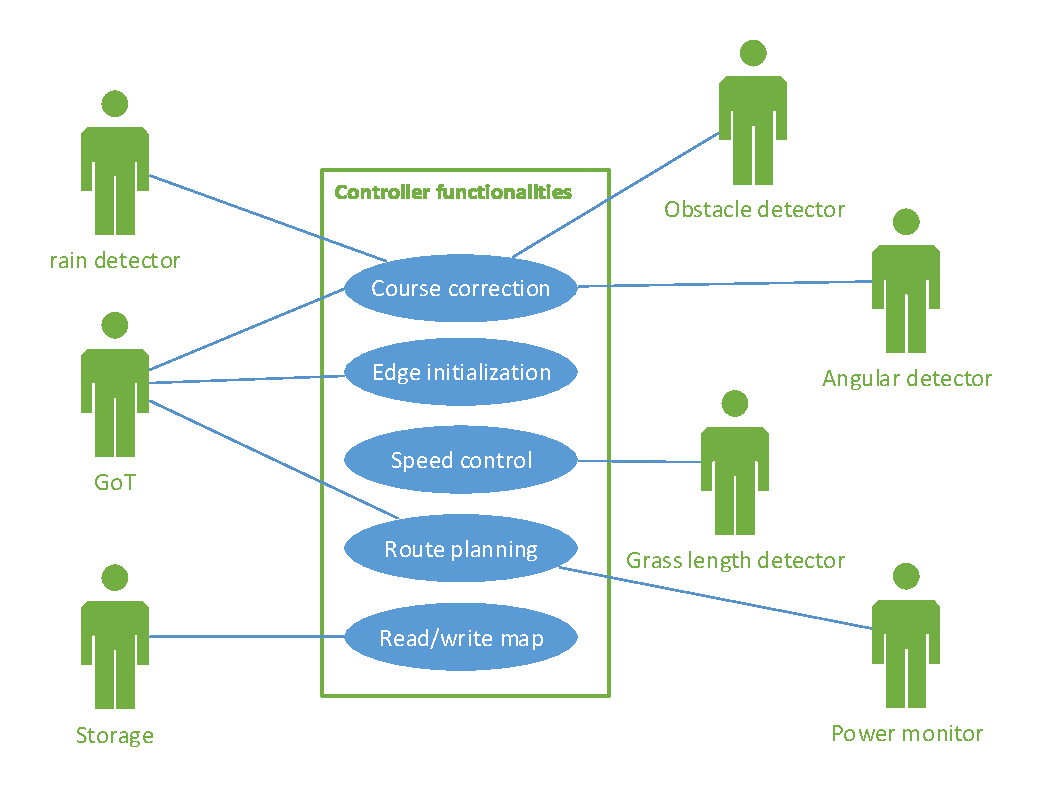
\includegraphics[scale=0.8]{figures/P5UseCase.pdf}
	\caption{Use-Case Diagram}
	\label{fig:usecase}
	\flushleft
\end{figure}

\noindent
The main purpose of the system is to automatically navigate in a specific area which is confined by the \textit{edge initialization} functionality. This functionality handles the marking of the areas edges. The functionality is only used in the initialization process of the system. The concept is to only use the functionality after the GoT system has been positioned in the area. The consumer then takes the system around the edges of the grass, while the GoT system tracks its positions. It is therefore only necessary to reinitialize the system, if the GoT satellites has been moved. While the edge is being tracked, the \textit{edge initialization} uses the \textit{read/write map} functionality to store the information collected, in storage. \\\\ 
\noindent
The route in which the lawn mower is to navigate, in the specified area, is provided by the functionality \textit{route planning}. \textit{Route planning} uses the information, about the specific area, which is collected from the storage, to plan the most optimal route. Furthermore the \textit{route planning} needs information about the systems power level to insure the functionality is considering if the system needs charging and therefore have to return to the charging station at some point on the route.\\\\
\noindent
The \textit{read/write map} functionality as described earlier, handles the communication with storage. Hence it stores information, received from the \textit{edge initialization} and collects information from storage when the functionality \textit{route planning} needs it. \\\\
\noindent
To insure the system is moving with a desired speed (in a straight line and in a turn) or a speed which is fitted to the height of the grass, detected with the \textit{grass length detector}, a \textit{speed control} functionality is necessary in the system to control the motors. To insure the \textit{speed control} can deliver the desired speed an \textit{angular sensor} is utilized. \\\\
\noindent
The last functionality, \textit{course correction} is used when the system strays of the path calculated by \textit{route planning} or if the path gets blocked.
The obstacle which is blocking the route is detected by the sensor \textit{obstacle detector}. Furthermore the GoT system and the \textit{angular detector} will detect if the system is not on the desired path, or if the system starts to slip. Also, if it starts to rain, which is detected by the \textit{rain detector}, the system has to return to the charging station.
Finally, the \textit{course correction} sends the calculated data to the functionality \textit{speed control}.

The overall functionalities of what the system must be able to do has been described. Now the different constraints on the system will be considered and the project prototype should be established.